% Two-panel diagram from Appendix A.1 of Yitian Chen, Agent Based Modeling for Group Alignment.
% Source: agent-based-modelling/paper.tex, commit 569dfe9483db20a30504b22692f7aa1957152659.
\begin{figure}[H]
    \centering
    \tikzset{
        cell/.style={draw=gray!70, minimum size=1.1cm, inner sep=0pt, font=\small},
        fast/.style={cell, fill=blue!25},
        slow/.style={cell, fill=orange!35},
        centre/.style={cell, fill=blue!70, text=white, font=\small\bfseries},
        offer/.style={-{Latex[length=2mm]}, thick},
        cnt/.style={font=\scriptsize, fill=white, inner sep=1pt}
    }
    %
    \begin{subfigure}[b]{0.36\textwidth}
        \centering
        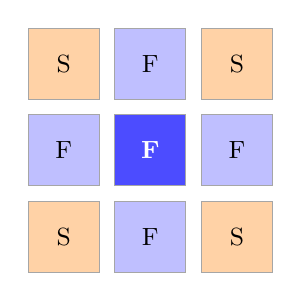
\begin{tikzpicture}
            \node[slow]   (nw) at (-1.1, 1.1) {S};
            \node[fast]   (n)  at ( 0,   1.1) {F};
            \node[slow]   (ne) at ( 1.1, 1.1) {S};
            \node[fast]   (w)  at (-1.1, 0)   {F};
            \node[centre] (c)  at ( 0,   0)   {F};
            \node[fast]   (e)  at ( 1.1, 0)   {F};
            \node[slow]   (sw) at (-1.1,-1.1) {S};
            \node[fast]   (s)  at ( 0,  -1.1) {F};
            \node[slow]   (se) at ( 1.1,-1.1) {S};
        \end{tikzpicture}
        \caption{Initial configuration: a fast agent (dark) with 4 fast (blue) and 4 slow (orange) neighbours.}
        \label{fig:app-neighbour-types}
    \end{subfigure}
    \hfill
    \begin{subfigure}[b]{0.58\textwidth}
        \centering
        \begin{tikzpicture}[x=2.5cm, y=2.5cm]
            \tikzset{cell/.append style={minimum size=0.9cm}}
            \node[slow]   (nw) at (-1, 1) {S};
            \node[fast]   (n)  at ( 0, 1) {F};
            \node[slow]   (ne) at ( 1, 1) {S};
            \node[fast]   (w)  at (-1, 0) {F};
            \node[centre] (c)  at ( 0, 0) {F};
            \node[fast]   (e)  at ( 1, 0) {F};
            \node[slow]   (sw) at (-1,-1) {S};
            \node[fast]   (s)  at ( 0,-1) {F};
            \node[slow]   (se) at ( 1,-1) {S};
            % fast <-> fast: rho offers each way (thick)
            \draw[offer, {Latex[length=2mm]}-{Latex[length=2mm]}, line width=1.4pt, blue!60!black] (c) -- (n) node[cnt, pos=0.32, right=2pt] {$\rho\,/\,\rho$};
            \draw[offer, {Latex[length=2mm]}-{Latex[length=2mm]}, line width=1.4pt, blue!60!black] (c) -- (s) node[cnt, pos=0.32, right=2pt] {$\rho\,/\,\rho$};
            \draw[offer, {Latex[length=2mm]}-{Latex[length=2mm]}, line width=1.4pt, blue!60!black] (c) -- (e) node[cnt, midway, above=2pt] {$\rho\,/\,\rho$};
            \draw[offer, {Latex[length=2mm]}-{Latex[length=2mm]}, line width=1.4pt, blue!60!black] (c) -- (w) node[cnt, midway, above=2pt] {$\rho\,/\,\rho$};
            % fast <-> slow: rho offers out, 1 back (thin)
            \draw[offer, {Latex[length=1.6mm]}-{Latex[length=1.6mm]}, line width=0.6pt, orange!70!black] (c) -- (nw) node[cnt, pos=0.68, above right=1pt] {$\rho\,/\,1$};
            \draw[offer, {Latex[length=1.6mm]}-{Latex[length=1.6mm]}, line width=0.6pt, orange!70!black] (c) -- (ne) node[cnt, pos=0.68, above left=1pt]  {$\rho\,/\,1$};
            \draw[offer, {Latex[length=1.6mm]}-{Latex[length=1.6mm]}, line width=0.6pt, orange!70!black] (c) -- (sw) node[cnt, pos=0.68, below right=1pt] {$\rho\,/\,1$};
            \draw[offer, {Latex[length=1.6mm]}-{Latex[length=1.6mm]}, line width=0.6pt, orange!70!black] (c) -- (se) node[cnt, pos=0.68, below left=1pt]  {$\rho\,/\,1$};
        \end{tikzpicture}
        \caption{Offers exchanged in one slow time step $dT_s$, written as (centre $\to$ neighbour)\,/\,(neighbour $\to$ centre). Each offer is accepted with probability $p$.}
        \label{fig:app-neighbour-offers}
    \end{subfigure}
    \caption{Local view of information exchange. A fast--fast pair exchanges $2\rho$ offers per slow time step while a fast--slow pair exchanges only $\rho+1$. For $\rho = 3$ that is $6$ against $4$; as $\rho$ grows the ratio $2\rho/(\rho+1) \to 2$.}
    \label{fig:app-communication-local}
\end{figure}
